\documentclass[a4paper, 12pt, notitlepage]{report}

\usepackage{amsfonts}  
\usepackage{graphicx}  
\usepackage{fullpage}
\usepackage[pagewise]{lineno}
\usepackage{hyperref}
\usepackage{longtable}                      
\usepackage{ltxtable}                       
\usepackage[usenames,dvipsnames]{color}
\usepackage{colortbl}          
\usepackage{tabularx, booktabs}   
\usepackage{multirow}
\usepackage{dirtree}
\definecolor{tableheadcolor}{gray}{0.8}
\definecolor{darkblue}{rgb}{0,0,.5}
\definecolor{gray}{gray}{0.95}
\definecolor{lightgray}{gray}{0.95}
\newcommand{\file}[1]{\textbf{#1}}
\newcommand{\state}[1]{{\tt\textbf{#1}}}
\newcommand{\signal}[1]{{\textbf{\tt#1}}}
\title{YAC - Yet Another CORDIC Core} 
\author{Christian Haettich [feddischson@gmail.com]} 
\date{\today}

\begin{document}

%%%%%%%%%% PRELIMINARY MATERIAL %%%%%%%%%%
\maketitle
\begin{center}
IP core and C-model documentation 
\end{center}
\thispagestyle{empty}

\tableofcontents 


\chapter{Organization and Introduction}
\section{History}
\begin{table}[htbp]
   \center
   \begin{tabular}{@{}llll@{}}
      \rowcolor{tableheadcolor}\textbf{Version}& \textbf{Date} & \textbf{Description} & \textbf{Author}  \\

      \multirow{1}{*}{0.02}  & 26th June 2018 & E-mail address update and diagrams de-drawn & Christian Haettich\\\midrule
      \multirow{1}{*}{0.01}  & 4th March 2014 & Initial document & Christian Haettich\\\midrule
      \bottomrule
   \end{tabular}
   \caption{History}
   \label{tab:frqband}
\end{table} 


\section{Folder and Files}

\dirtree{%
.1 /.
.2 c\_octave.
.3 cordic\_iterative.c\DTcomment{C-code for bit accurate model}.
.3 cordic\_iterative\_code.m\DTcomment{Script to auto-generate VHDL and C-code}.
.3 cordic\_iterative\_test.m\DTcomment{YAC performance analysis script}.
.2 doc.\DTcomment{Contains files to create this documentation}.
.2 licenses.
.3 lgpl-3.0.txt\DTcomment{LGPL license}.
.2 README.txt\DTcomment{A short read-me file}.
.2 rtl.
.3 vhdl.
.4 cordic\_iterative\_int.vhd\DTcomment{Top-level VHDL file}.
.4 cordic\_iterative\_pkg.vhd\DTcomment{VHDL package file}.
.4 cordic\_iterative\_tb.vhd\DTcomment{VHDL testbench}.
}

\section{License}
Copyright (c) 2014, Christian Haettich, All rights reserved. \newline\newline 
YAC is free software; you can redistribute it and/or               
modify it under the terms of the GNU Lesser General Public         
License as published by the Free Software Foundation; either       
version 3.0 of the License, or (at your option) any later version. \newline\newline
YAC is distributed in the hope that it will be useful,             
but WITHOUT ANY WARRANTY; without even the implied warranty of     
MERCHANTABILITY or FITNESS FOR A PARTICULAR PURPOSE.  See the GNU  
Lesser General Public License for more details.              \newline\newline
You should have received a copy of the GNU Lesser General Public   
License along with this library. If not, download it from          
http://www.gnu.org/licenses/lgpl                                   


\section{The CORDIC algorithm}

The CORDIC algorithm is used to do trigonometric, hyperbolic, multiplication 
and division calculations in a hardware-efficient way. This means, that
only bit-shift, addition and subtraction operations in combination
with a lookup-table is required.\newline
Good introductions are available in \cite{survey}\cite{vlsi}\cite{dawid}.
A description on wikibook.org \cite{wikibook} is also useful.
For this reason, no more introduction is given here and the following chapters assume, that
the reader is familiar with the CORDIC algorithm.


\chapter{IP-Core Description}

The two files \file{cordic\_iterative\_int.vhd} and \file{cordic\_iterative\_pkg.vhd}
implements an iterative CORDIC algorithm in fixed-point format. 
Iterative means, that the IP-core is started with a set of input data and after
a specific amount of clock cycles, the result is available. No parallel data
can be processed. The 
following six modes are supported:
\begin{itemize}
   \item trigonometric rotation
   \item trigonometric vectoring
   \item linear rotation
   \item linear vectoring
   \item hyperbolic rotation
   \item hyperbolic vectoring
\end{itemize}

\section{Port Description}
\begin{table}[htbp]
   \center
   \begin{tabular}{@{}lllll@{}}
      \rowcolor{tableheadcolor}\textbf{Name}& \textbf{Type} & \textbf{Direction} & \textbf{Size} & \textbf{Description} \\

      \multirow{1}{*}{clk}    & std\_logic         & input  & 1 & clock              \\\midrule
      \multirow{1}{*}{rst}    & std\_logic         & input  & 1 & synchronous reset  \\\midrule
      \multirow{1}{*}{en}     & std\_logic         & input  & 1 & clock-enable       \\\midrule
      \multirow{1}{*}{start}  & std\_logic         & input  & 1 & start trigger      \\\midrule
      \multirow{1}{*}{done}   & std\_logic         & output & 1 & done indicator     \\\midrule
      \multirow{1}{*}{mode}   & std\_logic\_vector & input  & 4 & mode configuration \\\midrule
      \multirow{1}{*}{x\_i}   & std\_logic\_vector & input  & XY\_WIDTH                & X input vector        \\\midrule
      \multirow{1}{*}{y\_i}   & std\_logic\_vector & input  & XY\_WIDTH                & Y input vector        \\\midrule
      \multirow{1}{*}{a\_i}   & std\_logic\_vector & input  & A\_WIDTH + 2             & angular input vector  \\\midrule
      \multirow{1}{*}{x\_o}   & std\_logic\_vector & input  & XY\_WIDTH + GUARD\_BITS  & X output vector       \\\midrule
      \multirow{1}{*}{y\_o}   & std\_logic\_vector & input  & XY\_WIDTH + GUARD\_BITS  & Y output vector       \\\midrule
      \multirow{1}{*}{a\_o}   & std\_logic\_vector & input  & A\_WIDTH + 2             & angular output vector \\\midrule
      \bottomrule
   \end{tabular}
   \caption{Port description}
   \label{tab:ports}
\end{table} 

\begin{figure}[p]
\centering
   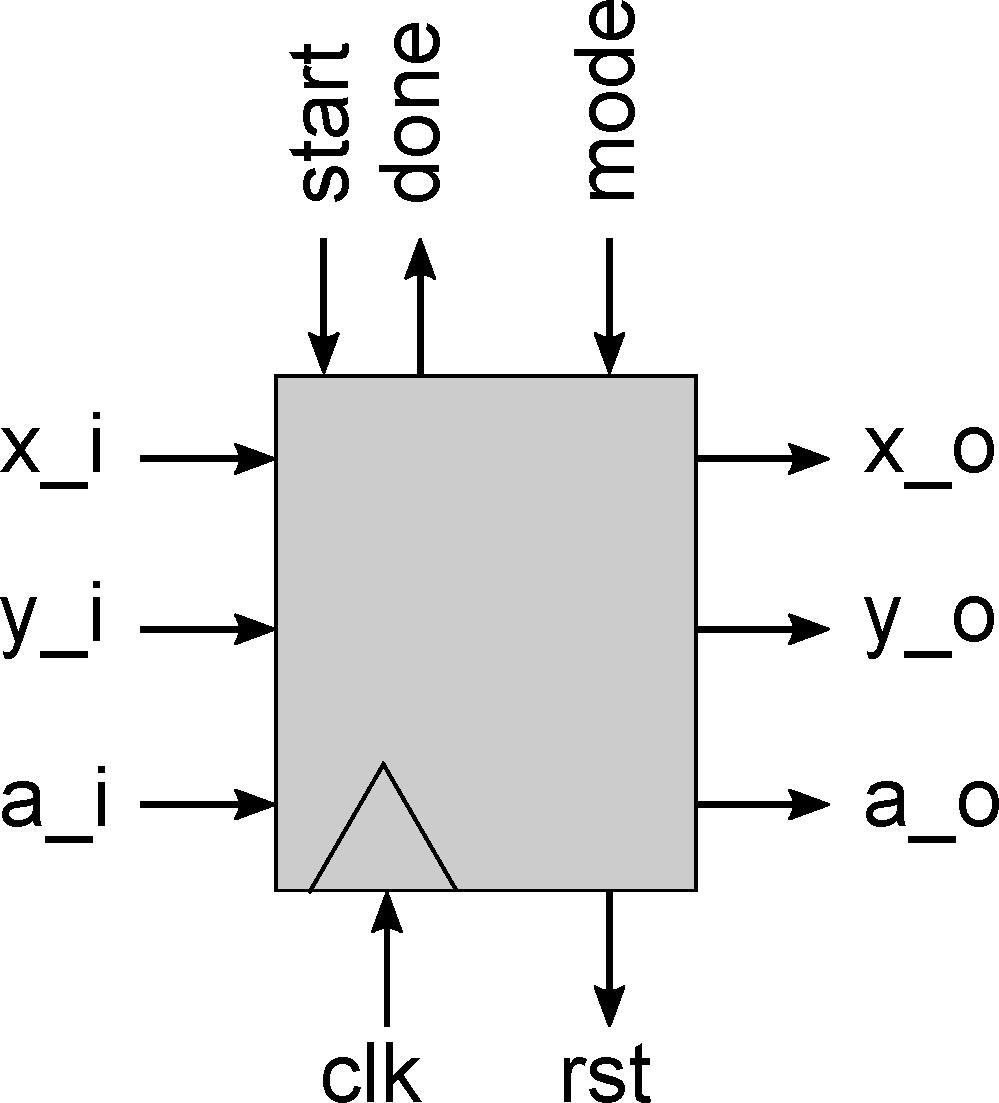
\includegraphics[width=250pt]{figs/block_symbol.pdf}
   \caption{YAC block symbol}
   \label{fig:ports}
\end{figure}
Table \ref{tab:ports} and Figure \ref{fig:ports} gives an overview
of the YAC ports.
The three input ports start, done and mode and are used to interact
with an external state machine or with a software driver.
After setting \signal{start} to high, the YAC starts processing.
If all necessary rotations are done, the \signal{done} output is set to 
high for one clock cycle.
When starting the YAC, all other inputs must contain valid data.
The mode input is used to select the CORDIC mode.
Table \ref{fig:ports} shows all input and output ports and Figure 
\ref{fig:ports} shows a CORDIC block symbol: $x_i, y_i, a_i, x_o, y_o, a_o$
are data ports whereas start, done and mode are configuration signals.






\section{Parameter Description}
\begin{table}[htbp]
   \center
   \begin{tabular}{@{}lllll@{}}
      \rowcolor{tableheadcolor}\textbf{Name}& \textbf{type} & \textbf{size} & \textbf{Description} \\

      \multirow{1}{*}{XY\_WIDTH}    & natural  & defines the size of x and y input and output vectors \\\midrule
      \multirow{1}{*}{A\_WIDTH}     & natural  & defines the size of the angular input and output vectors \\\midrule
      \multirow{1}{*}{GUARD\_BITS}  & natural  & defines the number of guard bits \\\midrule
      \multirow{1}{*}{RM\_GAIN}     & natural  & defines the precision of the CORDIC gain removal \\\midrule
      \bottomrule
   \end{tabular}
   \caption{Parameter description}
   \label{tab:params}
\end{table} 
Table \ref{tab:params} shows the four parameter, which can be used to parameterize 
the YAC.


\section{Mode description}
With the mode-input, it is possible to select between circular, linear and hyperbolic 
operation as well as between rotation and vectoring operations:
\begin{itemize}
\item mode(1:0) = "00" selects circular operation
\item mode(1:0) = "01" selects linear operation
\item mode(1:0) = "10" selects hyperbolic operation
\item mode(1:0) = "11" is reserved
\item mode(3) = '0' selects rotation
\item mode(3) = '1' selects vectoring
\end{itemize}
The package cordic\_iterative\_int.vhd contains the following defines to
setup the mode:
\begin{itemize}
   \item VAL\_MODE\_CIRC = "00" 
   \item VAL\_MODE\_LIN  = "01" 
   \item VAL\_MODE\_HYP  = "10" 
   \item I\_FLAG\_VEC\_ROT = 3 (bit index)
\end{itemize}
For example if a hyperbolic rotation mode is required, the mode input is "0010", 
and for the linear vector operation, the mode input is "1001".
Please note, that bit number 2 is reserved for future implementations.\newline
Table \ref{tab:modes} defines the behaviour of the YAC 
for different mode configurations.
\begin{table}[htbp]
   \center
   \begin{tabular}{@{}ll@{}}
      \rowcolor{tableheadcolor}\textbf{Setup}& \textbf{Description} \\

      \multirow{2}{*}{mode =( FLAG\_VEC\_ROT = 1, VAL\_MODE\_CIR ) } & $a_o = \textrm{atan2}( y_i, x_i ) \cdot \beta,  $\\
                                                                     & $x_o = \sqrt{ x_i^2+y_i^2 }  $ \\\midrule 
      \multirow{2}{*}{mode =( FLAG\_VEC\_ROT = 0, VAL\_MODE\_CIR ) } & $x_o = \cos( a_i / \beta ) \cdot \alpha  $\\
                                                                     & $y_o = \sin( a_i / \beta ) \cdot \alpha  $\\\midrule 
      \multirow{1}{*}{mode =( FLAG\_VEC\_ROT = 1, VAL\_MODE\_LIN ) } & $a_o = z + y/x $\\\midrule
      \multirow{1}{*}{mode =( FLAG\_VEC\_ROT = 0, VAL\_MODE\_LIN ) } & $a_o = y + x\cdot z  $ $  $\\\midrule
      \multirow{2}{*}{mode =( FLAG\_VEC\_ROT = 1, VAL\_MODE\_HYP ) } & $a_o = \textrm{tanh}( y_i / x_i ) \cdot \beta,   $\\
                                                                     & $x_o = \sqrt{ x_i^2-y_i^2 }                                 $\\\midrule 
      \multirow{2}{*}{mode =( FLAG\_VEC\_ROT = 0, VAL\_MODE\_HYP ) } & $x_o = \cosh( a_i / \beta ) \cdot \alpha$\\
                                                                     & $y_o = \sinh( a_i / \beta ) \cdot \alpha$\\
      \bottomrule
   \end{tabular}
   \caption{Mode description (see equation \ref{eqn:alpha} and \ref{eqn:beta} for $\alpha$ and $\beta$)}
   \label{tab:modes}
\end{table} 


\section{Data Range and Limitations}

   Both, the $x_i$ and $y_i$ inputs are defined with a size of $XY\_WIDTH$ and therefore,
   the maximum positive value in the two's complement format is
   \begin{eqnarray}
   \alpha & = & 2^{XY\_WIDTH-1}-1
   \label{eqn:alpha}
   \end{eqnarray}
   The angle input $a_i$ is defined with a size of $A\_WIDTH+2$.
   The value $\beta$ is defined with
   \begin{eqnarray}
   \beta & = & 2^{A\_WIDTH-1} -1
   \label{eqn:beta}
   \end{eqnarray}

   \subsection{Circular Vectoring Mode}

      The valid input range for $x_i$ and $y_i$ is $-\alpha ... +\alpha$.
      The angular input $a_i$ is ignored.

   \subsection{Circular Rotation Mode}
      The valid input range for $x_i$ and $y_i$ is $-\alpha ... +\alpha$.
      For the angular input $a_i$, values between $-\beta\pi$ and $+\beta\pi$ are valid.
      For calculating a complex rotation of a complex vector, all three inputs
      are required. For calculating $\sin$ and $\cos$, $x_i$ is set to $\alpha$
      and $y_i$ to 0, the angle input $a_i$ gets the angle.

   \subsection{Linear Vectoring Mode}
      The linear vectoring mode is used to calculate $y_i / x_i$. The limitation
      of this operation is the following:
      \begin{eqnarray}
         \frac{y_i}{x_i} \le 2
      \end{eqnarray}
      The valid input values for $x_i$ and $y_i$ are $-\alpha ... +\alpha$.

   \subsection{Linear Rotation Mode}
      The two inputs $x_i$ and $y_i$ have a valid data range between $-\alpha$ and $+\alpha$.


   \subsection{Hyperbolic Vectoring Mode}
      The data-range for $x_i$ and $y_i$ is $-0.79 \cdot \alpha$ to $0.79 \cdot \alpha$.


   \subsection{Hyperbolic Rotation Mode}
      The data-range for $a_i$ is $-\beta ... \beta$. Typically, $x_i$ is set to 
      $\alpha$ and $y_i$ to 0.

\section{Internal Operation}
\begin{figure}[p]
\centering
   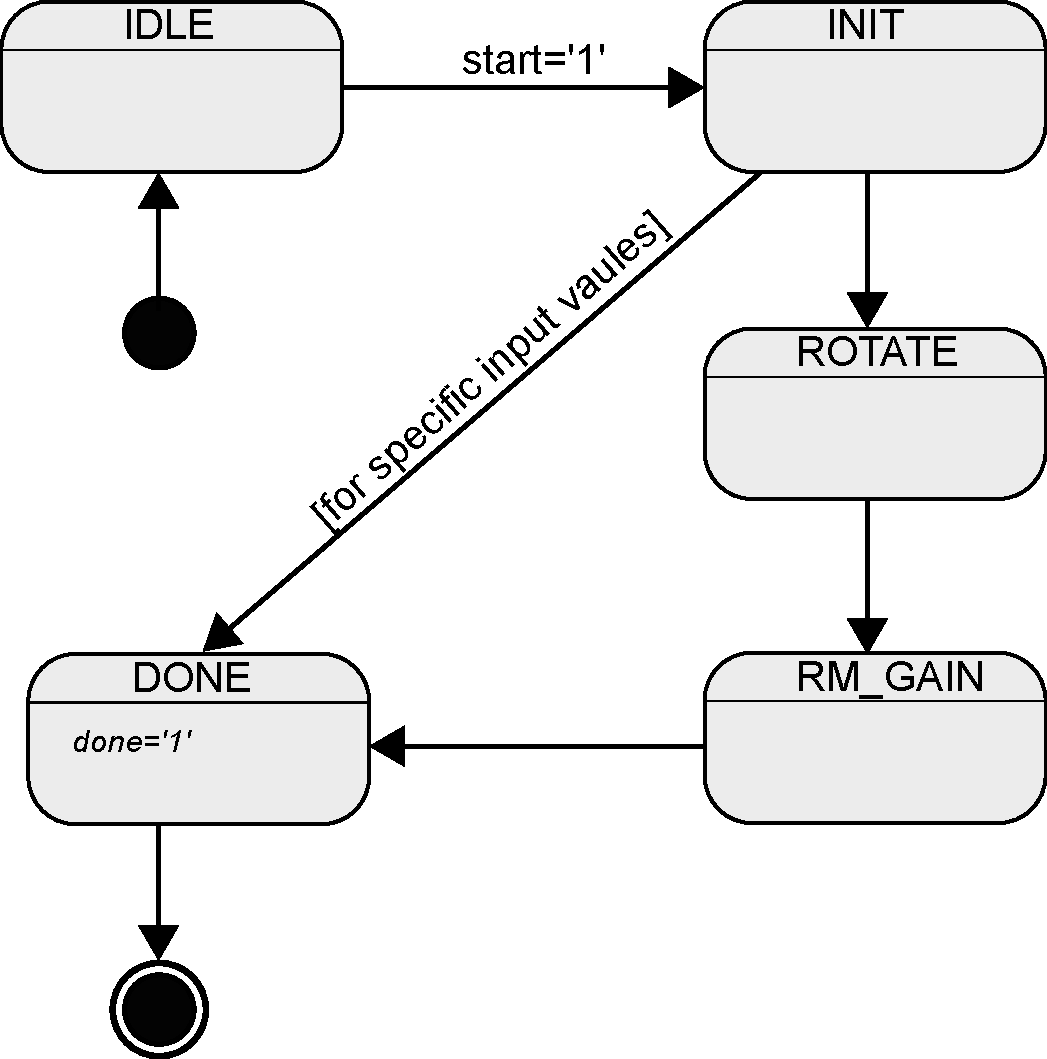
\includegraphics[width=300pt]{figs/state_diagram.pdf}
   \caption{State diagram}
   \label{fig:states}
\end{figure}
Five states are used do to the CORDIC algorithm. The five states are visualized in a
state diagram in Figure \ref{fig:states}.
After reset, the YAC goes into the \state{ST\_IDLE} state. Only in this state, the 
start signal is accepted. After starting the YAC, the state switches from
the \state{ST\_IDLE} state to the \state{ST\_INIT} state. The init state does some initial 
rotations/flipping.
After initialization, the main rotation starts with the \state{ST\_ROTATION} state
(there are a few cases, where no further rotations are required, see next sections).
Every rotation step is done within two clock cycles: in the first cycle, 
the angular value is loaded from the lookup-table and shifted. In addition, 
the x and y values are shifted. In the second
clock cycle, the results are added according to the CORDIC algorithm.
After all required iterations are done, the state switches to
the \state{RM\_GAIN} state, where the CORDIC gain is removed (depending on 
the mode). The last state \state{ST\_DONE} is only used to set the done flag to 
'1' for one clock cycle. After this, the YAC returns to the \state{ST\_IDLE} state.



   \subsection{Initialization}
   During the initialization state ST\_INIT, pre-rotations are done, depending on 
   the selected mode.


      \subsubsection{Circular Vectoring Mode}
      Because we support atan2 and not atan, we do the following pre-rotations. 
      Some specific input values don't need a further processing, for 
      example $atan( 0, 0 )$.\newline\newline
         \begin{tabular}{@{}lp{380pt}@{}}
            \rowcolor{tableheadcolor}\textbf{Input} &\textbf{ Description }  \\

            $x_i = 0, y_i = 0$    &    Fixed result: $x_o =  0, a_o = 0$,   
            to support cartesian to polar coordinate transformations, 
            further processing is skipped  \\ \midrule

            $x_i = 0, y_i > 0 $   &    Fixed result: $x_o =  y_i, a_o = \pi/2$,  
            further processing is skipped \\ \midrule

            $x_i = 0, y_i < 0 $   &    Fixed result: $x_o = -y_i, a_o = -\pi/2$,  
            further processing is skipped \\ \midrule


            $x_i < 0, y_i < 0 $   &    Pre-rotation from the third to the first quadrant,
                                       the angular register is initialized with $-\pi$ and
                                       the sign of the $x$ and $y$ register is flipped. \\ \midrule

            $x_i < 0, y_i \ge 0 $   &    Pre-rotation from the second to the fourth quadrant,
                                       the angular register is initialized with $\pi$ and
                                       the sign of the $x$ and $y$ register is flipped. \\ \midrule


            $x_i = + \alpha, y_i = + \alpha $   &  Fixed result: $x_o = \sqrt{2} \cdot \alpha, a_o = \frac{\pi}{4} \cdot \beta$ ,
            further processing is skipped \\ \midrule

            $x_i = + \alpha, y_i = - \alpha $   &  Fixed result: $x_o = \sqrt{2} \cdot \alpha, a_o = - \frac{\pi}{4} \cdot \beta$, 
            further processing is skipped \\ \midrule

            $x_i = - \alpha, y_i = + \alpha $   &  Fixed result: $x_o = \sqrt{2} \cdot \alpha, a_o =  \frac{3 \pi}{4} \cdot \beta$, 
            further processing is skipped \\ \midrule

            $x_i = - \alpha, y_i = - \alpha $   &  Fixed result: $x_o = \sqrt{2} \cdot \alpha, a_o = - \frac{3 \pi }{4} \cdot \beta$ ,
            further processing is skipped \\ 
            \bottomrule
         \end{tabular}

      \subsubsection{Circular Rotation Mode}
      The following pre-rotations are done:\newline\newline
         \begin{tabular}{@{}lp{380pt}@{}}
            \rowcolor{tableheadcolor}\textbf{Input} &\textbf{ Description }  \\

            $a_i < - \frac{\pi}{2}$    & Pre-rotation from the third to the first quadrant, 
                                         the sign of the $x$ and $y$ register is flipped, 
                                         the angular register is initialized with $\pi$   \\ \midrule

            $a_i >   \frac{\pi}{2}$    & Pre-rotation from the second to the fourth quadrant, 
                                         the sign of the $x$ and $y$ register is flipped, 
                                         the angular register is initialized with $-\pi$   \\
            \bottomrule
         \end{tabular}

      \subsubsection{Linear Vectoring Mode}
      The following pre-rotations are done:\newline\newline
         \begin{tabular}{@{}lp{380pt}@{}}
            \rowcolor{tableheadcolor}\textbf{Input} &\textbf{ Description }  \\

            $x_i < 0$          & Pre-rotation from the left half to the right half, thus
                                 the sign of the $x$ and $y$ register is flipped \\
            \bottomrule
         \end{tabular}


   \subsection{Rotation}

   \subsubsection{Hyperbolic Repetitions}
   The following iteration steps are repeated for convergence of the hyperbolic mode:
   \begin{eqnarray}
      4, 13, 40, 121, ..., 3i+1
   \end{eqnarray}



\section{Testbench}
A VHDL testbench (cordic\_iterative\_tb.vhd) is available which reads from an input file
data. This data is fed into the YAC. In addition, the input file must
provide the output data, which is expected from the YAC processing.
The following format is used in the testbench input-file:
\begin{verbatim}
x_i     y_i    a_i   x_o   y_o   a_o   mode

1234   1234   1234  1234  1234  1234    111  \
2345   2345   2345  2345  2345  2345    222  |  7 columns:
3456   3456   3456  3456  3456  3456    333  |  3 input, 3 output and one mode
...    ...                                   |
...                                          |
...
\end{verbatim}
The data must be in the two's complement with a base of 10.
After processing all lines, the testbench prints some info, how much
tests failed.\newline
For generating the test-patterns, the C-model with octave is used. By running
the script \file{cordic\_iterative\_test.m}, an entry 
in the testbech data file is done for every cordic calculation.


\chapter{Using the C-Model with Octave or Matlab}
For using the C-model, open octave or Matlab and compile the C-Model
with \newline
\textit{mex cordic\_iterative.c}
Afterwards, the C-model can be used in Octave/Matlab with the function call\newline
{\tt [ x\_o, y\_o, a\_o, it ] = cordic\_iterative( x\_i, y\_i, a\_i, mode, XY\_WIDTH, ANGLE\_WIDTH,
GUARD\_BITS, RM\_GAIN )}.\newline
The input and output arguments reflect almost the ports and parameters of the 
VHDL toplevel implementation, except that there is no done, start clk and rst port 
in the C-model. In addition, the last argument provides the number of iterations,
which are done.\newline \newline
The input arguments x\_i, y\_i, and a\_i can be 1xN vectors with N elements.
In this case, this three input arguments must have the same size. All
output arguments will also have the same size 1xN.



\section{Guard-Bits -- Input and output sizes}
It is possible to define MSB guard bits.
The need of MSB guard bits have several reasons. On the one hand,
they are required to handle the data growth of the cordic gain within the rotation state.
(which is compensated later). A nother reason is the data growth caused by the choise of
input data. For example 
\begin{eqnarray}
   \sqrt{ \alpha^2 + \alpha^2 } = \sqrt{2} \alpha
\end{eqnarray}
and therefore, a growth by the factor $\sqrt{2}$ happens, if an absolute calculation
of the two maximum input values is processed.\newline
\newline
Another point is the input and output size of the angular values ($a_i$ and $a_o$)
Because within this YAC, $\beta$ represents the angle 1, the input and output with
of $a_i$ and $a_o$ is A\_WIDTH+2, which allows to process angle values within
$-\pi ... \pi$


\subsection{Input data width versus iterations}
The number of iterations depends on the width of the input data. 
Input data with $X$ bit require $X+1$ rotations \cite{dawid}.
This requires, that the number of iterations are adapted. One solution might
be to detect the size of the input data and use this information for the CORDIC processing.
In YAC, a different sheme was chosen: the rotations are done until 
\begin{itemize}
   \item the angular register is 0 or doesn't change (in case of the rotation mode) 
   \item the y register is 0 or doesn't change (in case of the vecotring mode).
\end{itemize}
This results in a dynamic iterations adaption, depending the the input data width.

\chapter{Performance}
The performance is evaluated through the matlab script \file{cordic\_iterative\_test.m}.


\chapter{Open issues and future work}

   \section{Next steps}
   \begin{itemize}
      \item Add YAC to a FPGA based System-on-Chip to prove 
            FPGA feasibility
      \item Performance optimization
         \item circuit optimizations
         \item numerical optimizations
   \end{itemize}

   \section{Future plans}
   \begin{itemize}
      \item Hyperbolic range extension
      \item Floating point CORDIC 
   \end{itemize}



%%%%%%%%%% BIBLIOGRAPHY %%%%%%%%%%
\begin{thebibliography}{9}

\bibitem{survey}
  Andraka, Ray; \textit{A survey of CORDIC algorithms for FPGA based computers}

\bibitem{vlsi}
   Hu, Yu Hen; \textit{CORDIC-Based VLSI Architectures for Digital Signal Processing}

\bibitem{wikibook}
  CORDIC on wikibook: \url{http://en.wikibooks.org/wiki/Digital_Circuits/CORDIC}

\bibitem{dawid}
   David, Herbert; Meyr, Heinricht; \textit{CORDIC Algorithms and Architectures} 
   \url{http://www.eecs.berkeley.edu/newton/Classes/EE290sp99/lectures/ee290aSp996_1/cordic_chap24.pdf}
\end{thebibliography}
\end{document}


